\chapter{Referencial Teórico}
\label{chap:refteorico}

Nesta seção será apresentada o embasamento teórico para desenvolvimento do projeto.

%================================================================================
\section{Sistemas de Visão Computacional}
\label{sec:sistemasVisaoArtificial}

Os sistemas de visão computacional estão presentes em diversas áreas, sendo elas medicina, análise de impressões digitais, sensoriamento remoto, robótica móvel, entre outras. O sucesso obtido pelo seu grande poder de utilização tem sido relevante para o constante desenvolvimento destas tecnologias.

Visão computacional foi definida como sendo o conjunto de técnicas computacionais para estimar ou explicitar as propriedades geométricas e dinâmicas do mundo tridimensional a partir de imagens \cite{alves2005estudo}.

Devido a crescente automatização dos processos produtivos, busca-se tornar os sistemas computacionais e de robótica capazes de tornar automática a execução de tarefas complexas \cite{rudek2001visao}.

Sabe-se que a visão é a principal forma de obtenção de informações do ambiente para a maioria dos seres vivos. A imagem é formada na mente a partir dos olhos, que funcionam como sensores de luminosidade, e é processada pelo cérebro que determina a ação a ser tomada. Por exemplo, em um movimento para se pegar um copo a visão tem papel fundamental junto com a coordenação motora \cite{alves2005estudo}. É perceptível que muitas ações realizadas no dia a dia são extremante complicadas de se fazer sem o advento da visão.

Para visão computacional, em lugar de olhos temos câmeras como sensores de obtenção de imagens digitais. Estas imagens passam por um processamento digital onde técnicas computacionais tiram as informações desejadas do ambiente, variando de acordo com o objetivo da aplicação. Para a robótica, é comum a utilização na identificação de objetos, localização e locomoção. Diversas técnicas de reconhecimento de imagens, tem sido apresentadas na literatura e geralmente são validadas através de protótipo de aplicações, pois em um ambiente industrial, raramente obtém-se as condições ideais de iluminação, contraste, posicionamento correto da peça, e do ângulo de obtenção da imagem, além de outros fatores externos que dificultam a interpretação de uma cena. Uma imagem digital pode conter várias informações, que deverão ser tratadas em diferentes etapas da produção. Estas informações impossibilitam que imagens diferentes possam ser tratadas de uma forma única, isto é, imagens diferentes possuem requisitos de programação diferentes \cite{rudek2001visao}.

Portanto, temos a primeira etapa de desenvolvimento e utilização de um sistema de visão computacional, a definição do problema. As demais etapas são: aquisição da imagem, pré-processamento, segmentação, identificação do objeto e reconhecimento de padrões, como visto na Figura~\ref{fig:acoesProcImagem}.

\begin{figure}[!hbtp]
  \centering
   \caption{Ações de Aquisição e Processamento de Imagem.}
    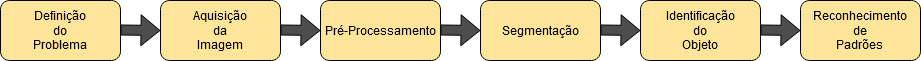
\includegraphics[width = 0.8\textwidth]{Caps/Figs/ref-teorico/acoes-procImagem.jpg}
   \label{fig:acoesProcImagem}
    \fonte{Autor}
\end{figure}

\subsection{Definição do Problema}
\label{subsec:defProblema}

Para \citeauthor{rogeralex1999} (\citeyear{rogeralex1999}), a primeira etapa do processo é a definição do problema, ou seja, qual é o objetivo que o sistema deve cumprir. Este pode ser a identificação de peças numa esteira rolante, a identificação de impressões digitais ou o reconhecimento de obstáculos na trajetória de um robô móvel. Se o sistema tiver sido bem planejado, chega-se a última etapa do processo, que é o resultado, ou seja, qual é a peça, a quem pertence a impressão digital ou qual é o obstáculo do robô.

\subsection{Aquisição da Imagem}
\label{subsec:aquisImagem}

Nesta etapa necessita-se de um dispositivo sensível a faixa do espectro eletromagnético desejado, também conhecido como câmera. Estes equipamentos que compõe o ambiente produzem em sua saída um sinal elétrico proporcional a quantidade de energia captada. Esse sinal elétrico, precisa então passar por um conversor analógico-digital para que possa ser processado pelo computador \cite{rogeralex1999}.

\subsection{Pré-processamento da Imagem}
\label{subsec:preProcImagem}

Após digitalizar e armazenar a imagem em um computador, as técnicas de pré-processamento são usadas para aprimorar a qualidade de uma imagem, corrigindo iluminação, contraste, distorções e nitidez~\cite{rudek2001visao}.

Essas operações podem ser realizadas tanto no domínio espacial quanto no domínio da frequência. O domínio espacial refere-se ao próprio plano da imagem e é caracterizado pela manipulação direta dos pixels. As técnicas de processamento no domínio da frequência são baseadas na manipulação da Transformada de Fourier da imagem~\cite{rogeralex1999}.

\subsection{Segmentação da Imagem}
\label{subsec:segImagem}

\citeauthor{heinen2004navegaccao} (\citeyear{heinen2004navegaccao}) afirma que em processamento de imagens, segmentar consiste em identificar e extrair estruturas homogêneas presentes em uma cena, sendo a eficiência deste processo diretamente relacionada ao desempenho final da análise automática de imagens. É importante enfatizar que essa é uma etapa crítica do processo.

Esta técnica é utilizada para reduzir o esforço computacional, reduzindo as informações da imagem. Para~\citeauthor{rudek2001visao} (\citeyear{rudek2001visao}), a ideia utilizada na segmentação (\textit{thresholding}) é dividir a imagem em regiões que correspondem a unidades estruturais da cena, ou que distinguem os objetos de interesse, separando os objetos da imagem (\textit{foreground}) das informações de fundo da imagem (\textit{background}). Com esta abordagem, minimiza-se o tamanho do espaço de onde as informações são retiradas, diminuindo o esforço computacional necessário para tratar a imagem.

A dificuldade normalmente encontrada está no fato de não haver conhecimento a priori do número e tipo de estruturas presentes na imagem. Estas são identificadas a partir de características como forma, geometria, topologia, textura, cor ou brilho, sendo escolhidas aquelas que possibilitam melhor distinção~\cite{heinen2004navegaccao}.

\subsection{Identificação do Objeto}
\label{subsec:idObjeto}

Visto que os elementos de interesse da imagem foram individualizados, deve-se determinar a melhor forma de representá-los, isto é, se apenas o seu contorno já contém a informação necessária ou se todos os pixels são necessários para a identificação do objeto. Portanto, deve-se determinar características do objeto que possam contribuir para a sua identificação.

\citeauthor{rudek2001visao} (\citeyear{rudek2001visao}) afirma que devido a uma variedade de razões, os dados de imagens usados na entrada de um sistema de visão, nem sempre são perfeitos. Os problemas que frequentemente ocorrem estão relacionados com a oclusão, onde um objeto pode estar parcialmente escondido atrás de outro objeto. 

De forma análoga, a perda de informações ou deformações, podem ser ocasionadas por ruídos na imagem devido a condições anormais de iluminação, defeitos de digitalização, e de resultados ineficientes de algoritmos de segmentação~\cite{beis1999indexing}.

\subsection{Reconhecimento de Padrões}
\label{subsec:recPadroes}

As técnicas de reconhecimento de padrões, tratam da identificação de partes da imagem que possuem semelhanças. Uma grande quantidade de ferramentas matemáticas e computacionais, tem sido desenvolvidas para permitir que objetos possam ser extraídos e agrupados em classes específicas de informações. Uma boa representação da forma do objeto, gera facilidades para que ele seja armazenado, transmitido, comparado, reconhecido ou mesmo entendido. A representação deve ser gerada de acordo com regras simples e precisas. Geralmente uma forma é descrita em termos de número de componentes, primitivas e relacionamentos entre estes componentes~\cite{rudek2001visao}.

%================================================================================
\section{OPENCV}
\label{sec:openCV}



%================================================================================
\section{Seção3}
\label{sec:EstimarF0}


 
